\chapter{专用电路设计与仿真}\label{chapter_design}
\graphicspath{{chapter4/figure/}}

通过一系列的算法测试,我们可以确认常规的DeSTIN算法在\uline{图像特征位置变化不明显}时进行静态、动态识别的准确度较高。 本章我们介绍基于DeSTIN算法,我们进行的\uline{单个神经元结构}的硬件设计工作:包括数据的量化测试、数字电路框架的设计以及数字电路的聚类测试仿真结果。

我们目前的硬件设计主要基于一个\uline{二维数据输入,内部四个聚类的单个神经元}。 

\section{定点数聚类测试}
采用定点数框架是因为其更容易在小型电路上实现,运算单元相对简单。大多数专用电路设计均采用定点数框架。

定点数测试是硬件设计的第一步。此时我们要将抽象的数转变为电路中的一组高低电平信号来考虑,将每一步算数运算考虑成电路中的一个逻辑运算单元。 尤其是对于乘法、除法,我们要考虑到牺牲精度后带来的影响以及溢出后是否较为严重地影响结果。

\subsection{定点数测试中注意的修改}
\subsubsection{数据的量化} 
在进行软件层次上的算法测试时,我们计算的对象都是$double$型双精度的浮点数;虽然浮点数运算过程复杂、耗费计算量,其运算范围广泛并且能够很好地保证精度,因而我们不用过于考虑算法具体实现上的“噪音”问题。

在我们今后的考虑中,不再有“数”这个抽象的概念。我们考虑的都是一组记录高电平、低电平的电线或者寄存器。我们进行每一步运算时,都要将其对应到底层高低电平的相互转换。

通过平衡计算资源与表示精度的需求,我们将数据的\textbf{二进制长度限制在16bit},也就是说,每一个数用16个高低电平来表示。 我们\textbf{小数位数控制为14位},并采用补码的编码方法,这样我们可以表示的数的范围便是:$-2\sim 1.999$,能够表示的最小精度是$6.1035*10^{-5}$。

采取补码进行运算时有很多"Trick",包括乘法、加法溢出的处理,正负数之间进行每一种运算的结果是否正确,在此不便赘述。

\subsubsection{运算合并与整理}
对于所有运算来说,最消耗计算资源、也是最消耗计算时间的计算之一便是除法。Fourier变换之所以能够产生快速算法,是因为其只涉及加法、乘法。我们希望在硬件设计之前,重新检查我们的算数运算内容,进行相应的整理、归并,减少运算次数,尤其是除法的运算次数。

首先,我们想到的是\uline{特定学习速率、饥饿速率的选择}的问题。当我们选择$\alpha = 0.125\;(=\dfrac{1}{8}),\beta = 0.125\;(=\dfrac{1}{8}), \gamma = 0.9844 \;(= 1- \dfrac{1}{64})$时,出现了大量的\uline{2的幂次},那么我们可以把所有的乘除法转化为左右移位的计算,省去了大量的计算复杂度。结合前面算法测试的经验,学习速率在这个范围以内对准确度不造成很大影响,也说明了这样处理的合理性。

其次,我们要检查残存除法的位置。 通过分析Online k-means聚类方法,我们发现其仍然有两部分存在除法:计算归一化距离$n$时每一个聚类存在一步除法(不可避免);最后计算Belief State时涉及大量除法。

当聚类数为4的时候,我们将计算Belief State的公式进行简化,有:

$$p_1 = \dfrac{\dfrac{1}{n_1}}{\dfrac{1}{n_1}+\dfrac{1}{n_2}+\dfrac{1}{n_3}+\dfrac{1}{n_4}} = \dfrac{n_2 n_3 n_4}{n_2 n_3 n_4 + n_1 n_3 n_4 + n_1 n_2 n_4 + n_1 n_2 n_3}$$

那么有:(我们用$a,b,c,d$作为下标)
\begin{equation}
p_a = \dfrac{n_b n_c n_d}{n_b n_c n_d + n_a n_c n_d + n_a n_b n_d + n_a n_b n_c}
\end{equation}

以上$a,b,c,d$可以轮换。我们只需先计算所有的三项乘积,计算其加和,再对每一个输出计算一次除法,除法的次数由2*J次缩减为J次。

\subsubsection{除法的实现: Cordic算法}

对于不可规避的除法,我们采用了一种Cordic(COordinate Rotation DIgital Computer)算法,这是一种空间资源消耗少的,简单易行的算法。 其基本原理基于一个三角函数公式:
\begin{equation}
\begin{aligned}
K_n R sin(\theta \pm \phi) & = & R sin(\theta) \pm 2^{-n} R cos(\theta) \\
K_n R cos(\theta \pm \phi) & = & R cos(\theta) \mp 2^{-n} R sin(\theta) \\
with K_n = \sqrt{1+2^{-2n}} & , & tan(\phi) = 2^{-n} 
\end{aligned}
\end{equation}

我们主要采用其在除法运算上的变体--属于"移位加"算法类的一种。主要思想是“多退少补”,不断将被除数右移,计算商更精确的位数。

我们将Cordic除法的MATLAB代码展示出来。
\begin{spacing}{1}
\begin{lstlisting}[language=Matlab][deletekeywords={input, beta, gamma}]
function zin = cordic_div(yin, xin)
%% Cordic Division Fixed Point Version
% By Pei Zeng, PHY, NJU, 05/12/2016
% numerictype: Ty = numerictype('WordLength',16,'FractionLength',14)
% NOTICE: the input divident yin should be SMALLER than the input division
% xin!!!

%% Testbench Setting
Ty = numerictype('WordLength',16,'FractionLength',14);  % for fixed point type
F = globalfimath('CastBeforeSum',0,'OverflowAction','Saturate',...
    'RoundingMethod','Floor', 'ProductMode','SpecifyPrecision'...    
    ,'ProductWordLength',16,'ProductFractionLength',14,... 
    'SumMode','SpecifyPrecision'...    
    ,'SumWordLength',16,'SumFractionLength',14);  % for global fixed math operation setting
P = fipref('NumberDisPlay','RealWorldValue','NumericTypeDisplay','full');  % for afterwards realworld number display

%% Cordic
iter = Ty.WordLength - 1;
% convert to fixed point if not
xin = fi(xin, Ty);
yin = fi(yin, Ty);
zin = fi(0, Ty);

for j=0:iter
        if(yin < 0)
                alpha = fi(1,Ty);
        else
                alpha = fi(-1,Ty);
        end
         
        y = yin + alpha * 2^(-j) * xin;
        z = zin - alpha * 2^(-j);
         
        %matrix(j+1,:) = [j yin alpha xin zin];
        
        yin = y;
        zin = z;
end
\end{lstlisting}
\end{spacing}


\subsection{定点数测试结果}
在做完以上修改后,我们重新在MATLAB平台上进行聚类测试。此处我们用到了MATLAB的定点仿真工具箱Fixed Point Toolbox,其用于模拟定点数的运算情况。我们将乘法溢出设置为"饱和",这样如果定点数相乘超过2,结果会停留在1.999的最大值上。这符合我们后面硬件计算的乘法设定。

进行定点数测试的代码如下:

\begin{spacing}{1}
\begin{lstlisting}[language=Matlab][deletekeywords={input, beta, gamma}]
%% MATLAB fixed point test -- Online Clustering
% Pei Zeng, PHY, NJU, 05/12/2016
% Testbench Setting
Ty = numerictype('WordLength',16,'FractionLength',14);  % for fixed point type
F = globalfimath('CastBeforeSum',0,'OverflowAction','Saturate',...
    'RoundingMethod','Floor', 'ProductMode','SpecifyPrecision'...    
    ,'ProductWordLength',16,'ProductFractionLength',14,... 
    'SumMode','SpecifyPrecision'...    
    ,'SumWordLength',16,'SumFractionLength',14);  % for global fixed math operation setting
P = fipref('NumberDisPlay','RealWorldValue','NumericTypeDisplay','full');  % for afterwards realworld number display


% Sample Generation
n=300;
x1 = 0.2; y1 = 0.6; sigma1x = 0.1; sigma1y = 0.1;
x2 = 0.2; y2 = 0.2; sigma2x = 0.1; sigma2y = 0.15;
x3 = 0.6; y3 = 0.2; sigma3x = 0.15; sigma3y = 0.1;
x4 = 0.6; y4 = 0.6; sigma4x = 0.05; sigma4y = 0.2;

samp1 = fi([x1 + sigma1x * randn(n,1),y1 + sigma1y * randn(n,1)],Ty);
samp2 = fi([x2 + sigma2x * randn(n,1),y2 + sigma2y * randn(n,1)],Ty);
samp3 = fi([x3 + sigma3x * randn(n,1),y3 + sigma3y * randn(n,1)],Ty);
samp4 = fi([x4 + sigma4x * randn(n,1),y4 + sigma4y * randn(n,1)],Ty);

sample = [samp1;samp2;samp3;samp4];

scatter(samp1(:,1),samp1(:,2));
hold on;
scatter(samp2(:,1),samp2(:,2));
hold on;
scatter(samp3(:,1),samp3(:,2));
hold on;
scatter(samp4(:,1),samp4(:,2));
hold on;

title('Fixed Point Test');
xlabel('xlabel');
ylabel('ylabel');
axis([-0.2,1,-0.2,1])

% parameter initialization
training = 1;   %Turn on the training switch
%alpha = 0.125; beta = 0.125; gamma = 0.9844;    %Learning Parameter
alpha = fi(0.125,Ty); beta = fi(0.125,Ty); gamma = fi(0.9844,Ty);    %Learning Parameter

% neuron Initialization
mu = fi(0.15 + 0.5 * rand(2,4),Ty);
sigma2 = fi(ones(2,4),Ty);
starve = fi(ones(4,1),Ty);

%Neuron Parameter Record
Mu1 = fi(zeros(4*n, 2),Ty); Sigma1 = fi(zeros(4*n, 2),Ty);
Mu2 = fi(zeros(4*n, 2),Ty); Sigma2 = fi(zeros(4*n, 2),Ty);
Mu3 = fi(zeros(4*n, 2),Ty); Sigma3 = fi(zeros(4*n, 2),Ty);
Mu4 = fi(zeros(4*n, 2),Ty); Sigma4 = fi(zeros(4*n, 2),Ty);
Starve = fi(zeros(4*n, 4),Ty);

sample = sample(randperm(4*n),:);

%Training Process
for t = 1:(4*n)
    input = sample(t,:)';
    [belief, mu, sigma2, starve] = OnlineClustering(input, mu, sigma2, starve, alpha, beta, gamma, training);
    Mu1(t,:) = mu(:,1)';
    Mu2(t,:) = mu(:,2)';
    Mu3(t,:) = mu(:,3)';
    Mu4(t,:) = mu(:,4)';
    Starve(t,:) = starve';
end

%Plot
for t = 1:(4*n)
    plot(Mu1(t,1),Mu1(t,2),'r.',Mu2(t,1),Mu2(t,2),'b.',Mu3(t,1),Mu3(t,2),'g.',Mu4(t,1),Mu4(t,2),'k.');
    hold on;
end

% Plot Ellipse
DrawEllipse(mu(:,1),sigma2(:,1));
DrawEllipse(mu(:,2),sigma2(:,2));
DrawEllipse(mu(:,3),sigma2(:,3));
DrawEllipse(mu(:,4),sigma2(:,4));

\end{lstlisting}
\end{spacing}

其中online聚类算法代码如下:
\begin{spacing}{1}
\begin{lstlisting}[language=Matlab][deletekeywords={input, beta, gamma}]
function [belief, mu, sigma2, starve] = OnlineClustering(input, mu, sigma2,starve, alpha, beta, gamma, training)
%% Use Online k-means Clustering method to calculate the belief
%% Fixed Point Version
% Written by Pei Zeng, PHY, NJU
% Date 2016/05/12

% Data input to this function: 
% input: input data to the neuron. I-by-1 vector 
% (I is the input dimension,which is defined in DeSTIN.m)
% mu: centroid attribute for the coordinate of center. I-by-J vector
% (J is the belief dimension, which is defined in DeSTIN.m)
% sigma2: centroid attribute for the radius square. I-by-J vector

% New data output from this function:
% belief: new belief state of the neuron: J-by-1 vector

% initialization
I = size(input,1);
J = size(mu, 2);

%% Testbench Setting
Ty = numerictype('WordLength',16,'FractionLength',14);  % for fixed point type
F = globalfimath('CastBeforeSum',0,'OverflowAction','Saturate',...
    'RoundingMethod','Floor', 'ProductMode','SpecifyPrecision'...    
    ,'ProductWordLength',16,'ProductFractionLength',14,... 
    'SumMode','SpecifyPrecision'...    
    ,'SumWordLength',16,'SumFractionLength',14);  % for global fixed math operation setting
P = fipref('NumberDisPlay','RealWorldValue','NumericTypeDisplay','full');  % for afterwards realworld number display

%% Data Processing
% 1. Calculating the Euclidean distance from the input to each centroid
D_Euc = fi(zeros(J, 1),Ty);
for j = 1 : J
    D_Euc(j) = (input - mu(:,j))' * (input - mu(:,j));
end

% 2. Judge which cluster the input belongs to: Winner-take-all method
[~, j0] = min(starve .* D_Euc);

if (training == 1) % do the renewing only in the training process
% 3. Renew the starvation trace of each centroid
starve = starve * gamma;
starve(j0) = starve(j0) + (fi(1,Ty) - gamma);

% 4. Calculate the error for the centroid j0 and the input signal
Er_mu = input - mu(:,j0);
Er_sigma2 = (input - mu(:,j0)).* (input - mu(:,j0)) - sigma2(:,j0);

% 5. Learning Process: learning rate : alpha, beta
mu(:,j0) = mu(:,j0) + alpha * Er_mu;
sigma2(:,j0) = sigma2(:,j0) + beta * Er_sigma2;
end

% 6. Calculate the Mahanalobis distance: IMPORTANT
D_Mah = fi(zeros(J, 1),Ty);
% cordic_div version
for j = 1 : J
    for i = 1 : I
        D_Mah(j) = D_Mah(j) + cordic_div( (input(i) - mu(i,j))*(input(i) - mu(i,j)), sigma2(i,j) );
    end
end

% 7. "Inverse-normalize" the D_Mah values, and attain the new belief state
Multi = fi(ones(J, 1), Ty);
for j = 1 : J
    for k = 1: J
        if (k~=j)
            Multi(j) = Multi(j) * D_Mah(k);
        end
    end
end

Sum = sum(Multi);

% Cordic_div version belief calculation
belief = fi(zeros(J, 1), Ty); 
for j = 1 : J
    belief(j) = cordic_div(Multi(j), Sum);
end

\end{lstlisting}
\end{spacing}

最终的聚类测试结果仍然较为理想。我们附上同第三章常规测试的结果如图\ref{fig:fixedre}和表\ref{tab:clustestfix}。

\begin{figure}[htbp]
   \centering
   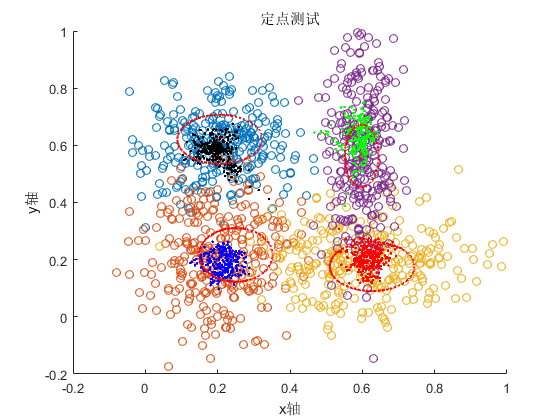
\includegraphics[width=0.7\textwidth]{FixedPointClustering.png} % requires the graphicx package
   \caption{定点测试:常规测试,结果图}
   \label{fig:fixedre}
\end{figure}

\begin{table}[htbp]
\centering
\begin{tabular}{c|c||c|c}
  \hline
  $\mu_{real}$   &  $\sigma_{real}$ &  $\mu$  &   $\sigma$\\
  \hline
  $(0.2,0.2)$    &  $(0.1,0.15)$   &  $(0.2501, 0.2169)$  & $(0.1172, 0.0859)$ \\
  $(0.2,0.6)$    &  $(0.1,0.1)$   &  $(0.2058, 0.6210)$  & $(0.1097, 0.0961)$ \\
  $(0.6,0.2)$    &  $(0.15,0.1)$   &  $(0.6271,0.1763)$  & $(0.0469, 0.1094)$ \\
  $(0.6,0.6)$    &  $(0.05,0.2)$   &  $(0.5983, 0.5628)$  & $(0.0573, 0.1648)$ \\
  \hline
\end{tabular}
\caption{定点聚类测试:聚类结果比较}
\label{tab:clustestfix}
\end{table}

对于$\sigma$误差过大,部分原因是我们运算中采用的是$\sigma^2$,因而上表得到的数据经过了一次定点数下的开方,而开放运算相当不准确。

在此有必要进行补充说明的是,我们是经历过多次数据量化方法的选择才最终确定“16位长度,14位小数”的结果的,所以说真实的调试过程是\uline{在"x位长度,y位小数"下进行MATLAB定点测试,最终因为较低精度,较少小数位导致结果不收敛或者报错;在尽可能少的位数要求下优化出了这个结果}。


\section{硬件结构设计}

我们通过定点测试得到了数据量化的基本要求以及除法的解决方案。接下来,我们进行了硬件的设计。

笔者将简要介绍自己设计的硬件结构的框架,然后介绍重要细节部分的实现方法;最终介绍细节部分的仿真结果。

\subsection{总体结构设计示意图}

如图\ref{fig:clusterframe},笔者采用Microsoft Visio进行制图。 整个硬件分为\textbf{神经单元,饥饿单元,比较器单元和信度计算单元}四个部分。

图\ref{fig:clusterframe}中每一列代表一个聚类,每一行代表一个输入数据维度;那么每一个聚类有I个神经单元和1个饥饿单元;总共J个聚类。每一个神经单元负责处理一个聚类某一维度的数据。

数据首先通过\uline{Input Bus}进入到每个神经单元,神经单元计算出其与data之间的Euclid距离后经\uline{Dist Bus}送入比较器,更新判断信号通过\uline{Renew Bus}返回到各个神经单元和饥饿单元,单元进行更新过程,并输出归一化Euclid距离,通过\uline{Ndist Bus}送至信度计算单元进行计算。

\begin{figure}[p]
   \centering
   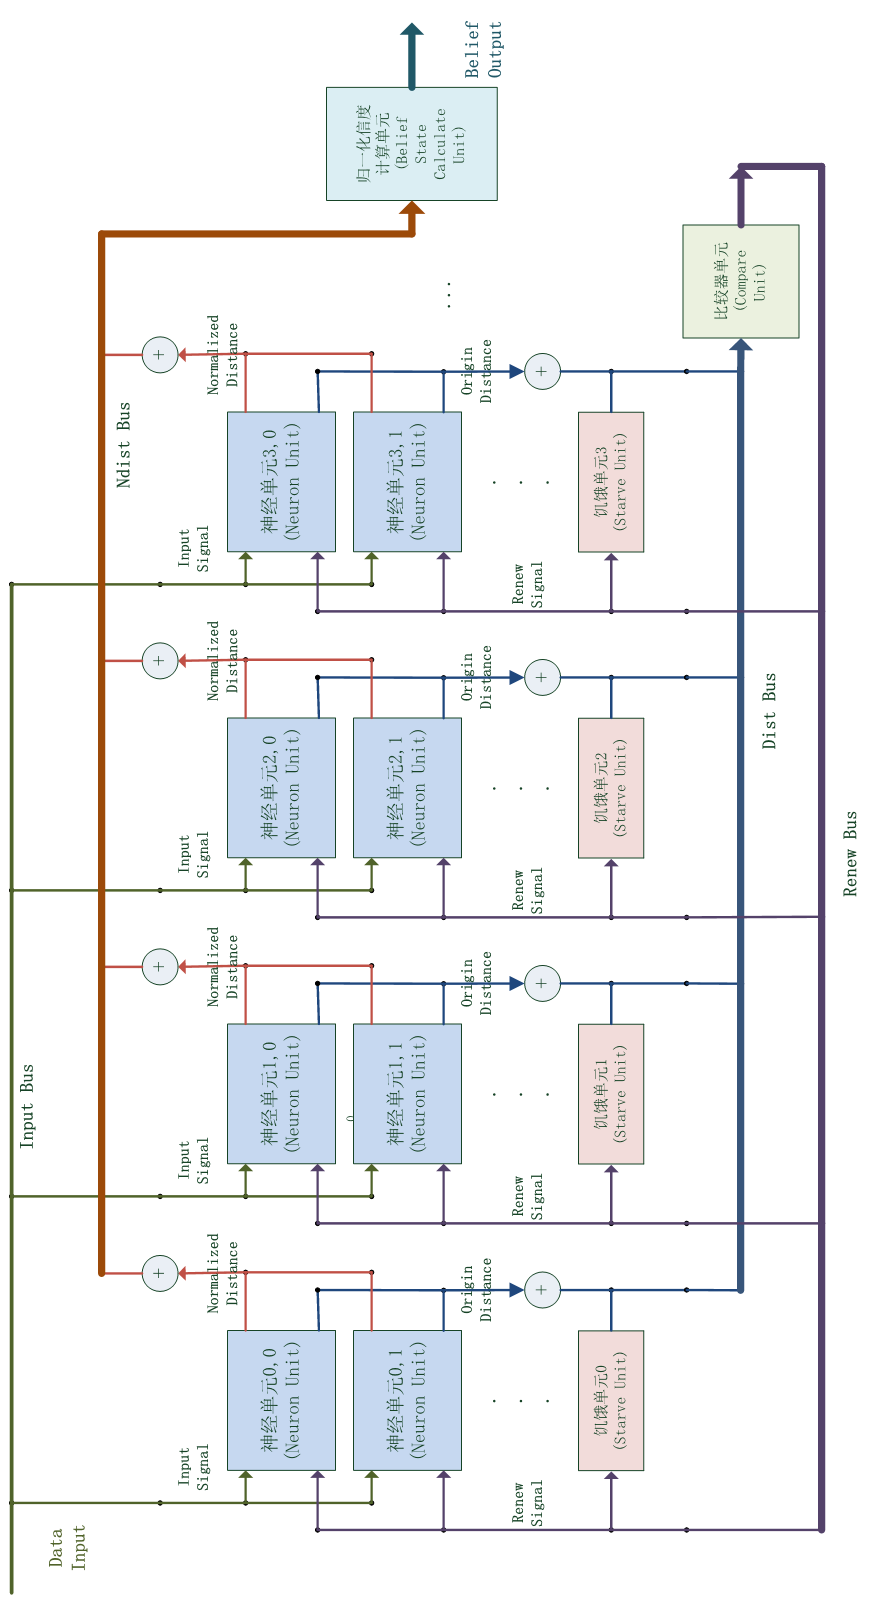
\includegraphics[width=0.8\textwidth]{ClusterStructure.png} % requires the graphicx package
   \caption{Online Clustering整体框架}
   \label{fig:clusterframe}
\end{figure}

\subsection{神经单元模块内部结构}
我们详细介绍神经单元Neuron Unit模块的设计。

如图\ref{fig:neuronunit},Neuron Unit外部引脚包括:
\begin{itemize}
\item 3个数据引脚(均为16bit):In, Mu-ini, Sigma2-ini,其中In接收观测数据输入,后面两个主要用于神经单元的参数初始化。

\item 3个使能端:En-input, En-renew, En-divide,分别进行其功能的主要阶段的控制:输入,计算dist;更新过程;计算ndist。使能端主要由外部的程序计数器控制(我们使用了有限状态机的方法)。

\item 2个判断信号: Ini-para, Renew-flag, 前一个用于是否初始化mu,sigma2的判断与信号选择;后一个由比较器返回,用于判断本次操作是否更新聚类参数mu,sigma2。

\item 2个底部引脚: Rst,Clk,其中一个为重置信号,另一个为时钟信号。

\item 3个输出引脚: Dist为单维度Euclid距离值输出;Ndist为单维度归一化Euclid距离值输出;Divide-flag为除法完成信号,用于后续步骤的指示。
\end{itemize}



\begin{figure}[htbp]
   \centering
   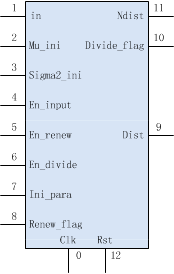
\includegraphics[width=0.2\textwidth]{NeuronUnit.png} % requires the graphicx package
   \caption{Neuron Unit外部引脚示意图}
   \label{fig:neuronunit}
\end{figure}

我们将其内部结构的实现通过Visio画出来,见\ref{fig:neuronunitlarge}。其中标注有“reg”的为内存器结构,上方引脚信号为使能端;“?”为路径选择器结构,上方引脚信号为选通信号;所有尖角正方形代表其为时序结构,底部引脚都要接上Rst,Clk;所有圆角或者圆形部分表示其为纯逻辑结构,应该在1个时钟周期内完成。

\begin{figure}[p]
   \centering
   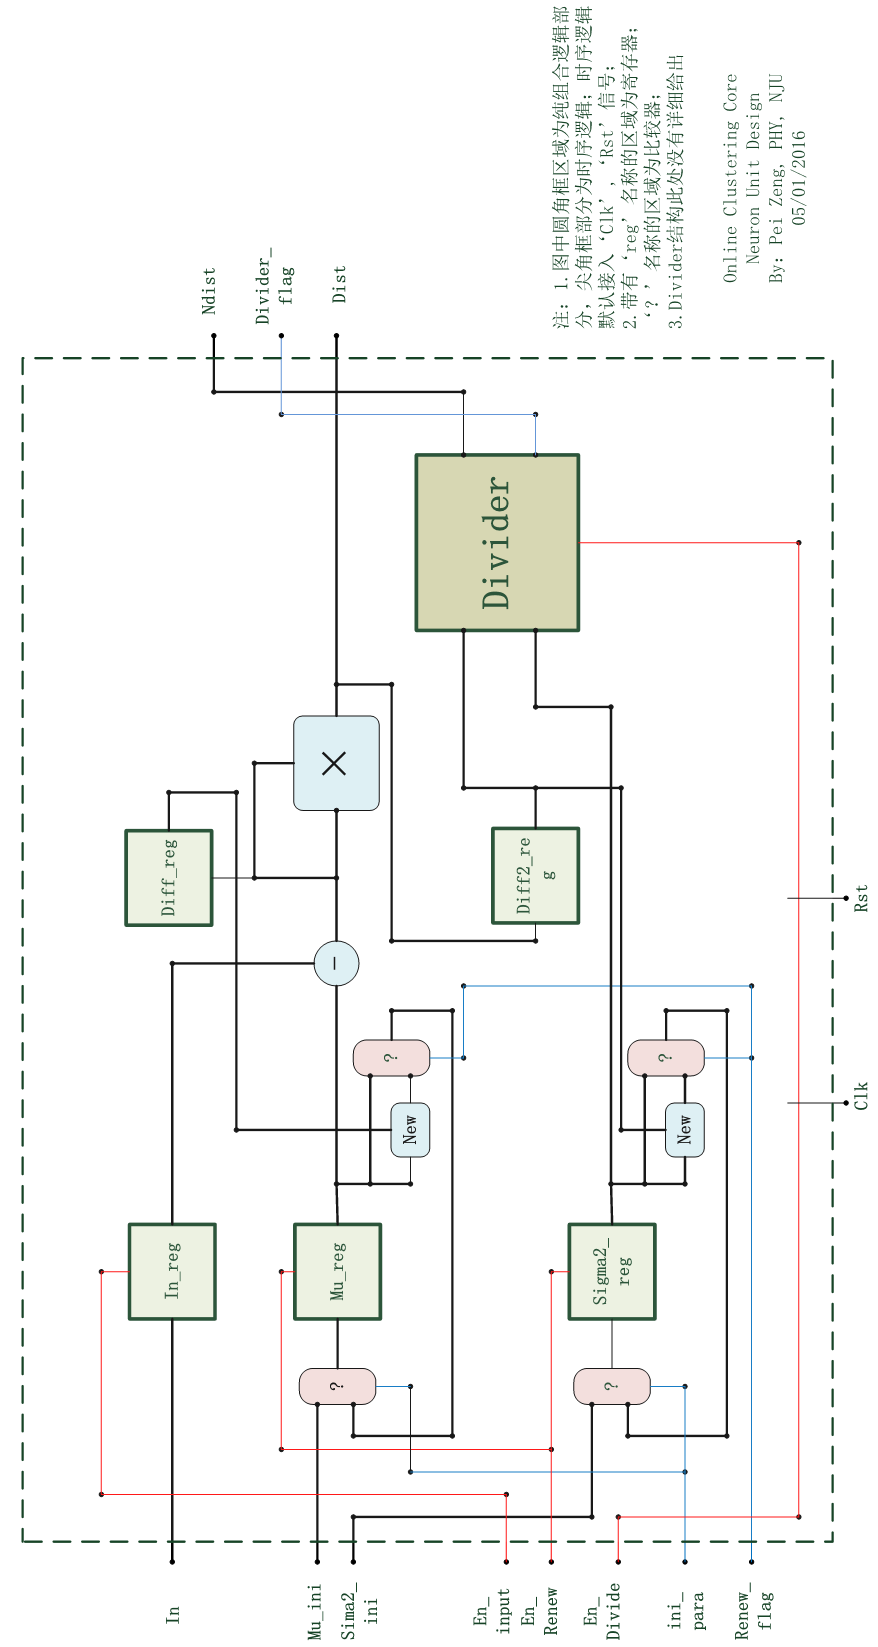
\includegraphics[width=0.8\textwidth]{NeuronUnitLarge.png} % requires the graphicx package
   \caption{Neuron Unit内部框架示意图}
   \label{fig:neuronunitlarge}
\end{figure}

我们不再详细介绍其他部分的结构,只将其Verilog代码附在附录里面。

\section{ModelSim仿真结果}
我们目前还没有完成对整个聚类的Modelsim仿真,只对每一个小部件进行了仿真。我们展示对于信度计算模块以及cordic除法器模块的仿真结果。

图\ref{fig:divsim}为除法器的仿真过程。我们测试了包括了正负数各种情况,较大与较小数相除等各种情况,确认了其除法的可靠性。(不能进行两个负数的除法;为了使其除法可靠,我们在除法器内部扩充了12位的辅助bit,参见附录Verilog代码)

\begin{figure}[htbp]
   \centering
   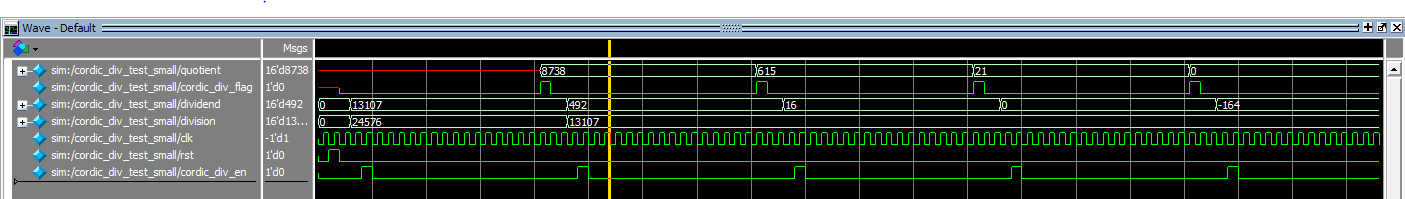
\includegraphics[width=0.8\textwidth]{DividerSim.png} % requires the graphicx package
   \caption{除法器的仿真结果}
   \label{fig:divsim}
\end{figure}


图\ref{fig:belisim}为信度计算模块的仿真过程。我们测试了十组参数,确认了其可靠信度计算的范围为:单个输入数据大于0.04,最高不超过1。(最高超过了影响不大,输入数据过小将导致结果错误)

\begin{figure}[htbp]
   \centering
   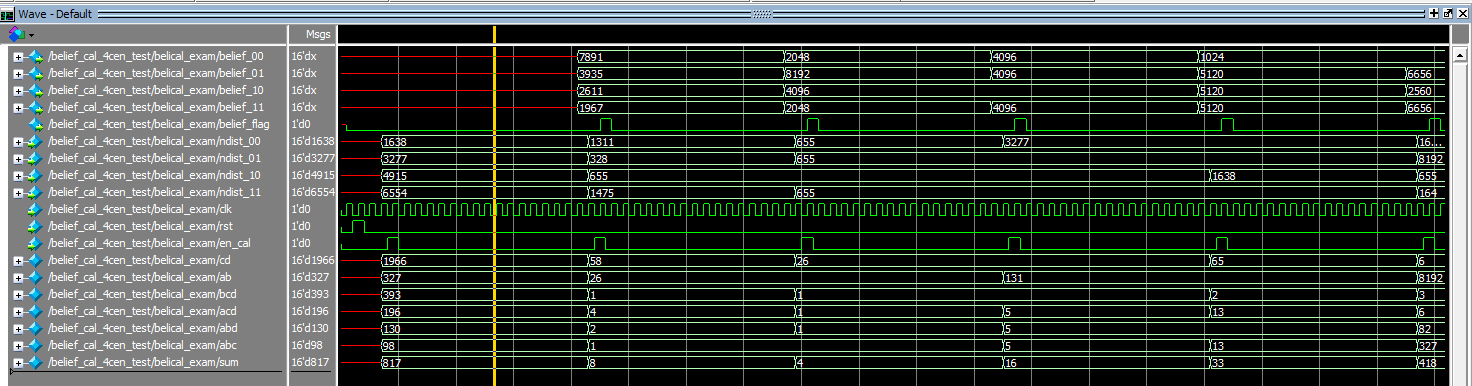
\includegraphics[width=0.8\textwidth]{BelicalSim.png} % requires the graphicx package
   \caption{信度计算的仿真结果}
   \label{fig:belisim}
\end{figure}

\subsection{现有问题与下一步的研究计划}
由于时间过短,笔者没有完成专用电路的整个设计流程。仍然有很多工作需要完成。

算法上,我们仍然没有解决特征空间位置移动时的时间空间特征识别的问题,我们将考虑结合卷积神经网络的方法,进行CTFAR测试以及动态识别的测试;

硬件上,我们仍然没有完成顶层模块的仿真工作(状态机设计有问题,数据量过于庞大);接下来我们要继续仿真工作,并进行综合排版布线,在FPGA上先进行测试,如果能够做到比较好的识别效果,可能会考虑进行流片工作。

